\documentclass[10pt]{book}
\usepackage[a5paper,top=54pt,bottom=54pt,left=48pt,right=48pt]{geometry}
\usepackage[utf8]{inputenc}
\usepackage[T1,T2A]{fontenc}
\usepackage[english,russian]{babel}
\usepackage{graphicx}
\usepackage{amsmath,amsthm,amssymb}
\usepackage{caption2}


%page header
\usepackage{fancybox,fancyhdr}
\pagestyle{fancy}
\fancyhead{}
\fancyhead[LE,RO]{\textbf{\thepage}}
\fancyhead[RE]{\textit{\textsection 47. Криволинейные интегралы}}
\fancyhead[LO]{\textit{47.5 Формула Грина}}
\fancyfoot{}
\renewcommand{\headrulewidth}{0pt}

\setcounter{page}{132}
\setcounter{figure}{149}

%remove colon after "Рис. %number%"
\renewcommand{\captionlabeldelim}{~}

%font
\fontfamily{lh}
\selectfont

\usepackage{pgfpages}
\pgfpagesuselayout{2 on 1}[a4paper,landscape,border shrink=5pt]

\begin{document}


    \small{Рассмотрим общий случай. Пусть область $G$ разбита на области \linebreak $G_{i}$, $i = 1, 2, \dots , k$, указанного в условиях теоремы вида. В силу до- \linebreak казанного для каждого $i = 1, 2, \dots , k$ \par

    $$\iint\limits_{G_{i}} \left( \dfrac{\partial Q}{\partial x} - \dfrac{\partial P}{\partial y} \right) dx dy = \int\limits_{\gamma^+_{i}} P dx + Q dy.$$

    \noindent Сложим эти равенства: \par

    $$\sum_{i=1}^{k} \iint\limits_{G_{i}} \left( \dfrac{\partial Q}{\partial x} - \dfrac{\partial P}{\partial y} \right) dx dy = \sum_{i=1}^{k} \int\limits_{\gamma^+_{i}} P dx + Q dy. \eqno (47.17)$$

    В силу аддитивности двойного интеграла по множествам \linebreak
    (см. п. 44.5) \par

    $$\mathbf{\sum_{i=1}^{k}} \iint\limits_{G_{i}} \left( \dfrac{\partial Q}{\partial x} - \dfrac{\partial P}{\partial y} \right) dx dy = \iint\limits_{G} \left( \dfrac{\partial Q}{\partial x} - \dfrac{\partial P}{\partial y} \right) dx dy$$


    В сумме, стоящей в правой части равенства (47.17), криволиней- \linebreak ные интегралы берутся дважды по всем внутренним частям границ \linebreak $\gamma_{i}$ областей $G_{i}$, т. е. таким частям кривых $\gamma_{i}$, которые являются \linebreak частью границ двух областей $G_{i}$, $i = 1, 2, \dots , k$ и, следовательно, не \linebreak входят в границу области $G$; при этом ориентации этих частей кривых \linebreak $\gamma_{i}$ противоположны (рис. 150). В силу изменения знака криволиней- \linebreak ного интеграла второго рода при изменении ориентации кривой сум- \linebreak ма двух криволинейных интегралов по указанным частям кривых \linebreak $\gamma_{i}$ равна нулю. Поэтому в правой сумме формулы (47.17) останутся \linebreak только интегралы по положению ориентированным частям грани- \linebreak цы $\gamma$ области $G$, дающие в сумме $\int\limits_{\gamma^+} P dx + Q dy$. Таким образом, \par

    $$\sum_{i=1}^{k} \int\limits_{\gamma^+_{i}} P dx + Q dy = \int\limits_{\gamma^+} P dx + Q dy. \eqno (47.18)$$

    Из формул (47.17) и (47.18) и следует формула (47.12) в общем \linebreak случае. \par
    Теорема доказана. \par
    Пусть $G$ --- ограниченная область плоскости $E^2$ и пусть ее \linebreak граница состоит из конечного числа простых контуров, которые \linebreak будем называть \textit{граничными контурами}. Если граничный контур \linebreak является одновременно и границей неограниченной области, лежа- \linebreak щей в $E^2 \diagdown \overline{G}$, то будем называть его \textit{внешним}, а если он является \linebreak одновременно границей ограниченной области, лежащей в $E^2 \diagdown \overline{G}$, \linebreak то --- \textit{внутренним}. Так, на рис. 151 контур $\gamma_{e}$ внешний, а контуры \linebreak $\gamma_{i1}$ и $\gamma_{i2}$ внутренние. \par

    Если граница области $G$ состоит из внешнего контура $\gamma_{e}$ и внут- \linebreak ренних контуров $\gamma_{i1}, \gamma_{i2}, \dots, \gamma_{im}$ и если область $G$ может быть раз- \linebreak бита на конечное число элементарных относительно обоих коорди- \linebreak натных осей областей с кусочно-гладкими границами, то справедлива \linebreak формула \par

    $$\iint\limits_{G} \left( \dfrac{\partial Q}{\partial x} - \dfrac{\partial P}{\partial y} \right) dx dy = \int\limits_{\gamma^+_{e}} P dx + Q dy + \sum_{j=1}^{m} \int\limits_{\gamma^-_{ij}} P dx + Q dy. \eqno (47.19)$$

    %pictures
        \begin{figure}[h]
        \begin{minipage}{0.45\textwidth}
        \centering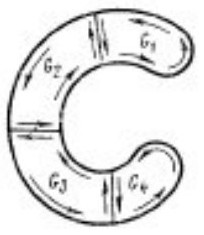
\includegraphics[width=60pt,height=100pt,keepaspectratio]{pic1}
        \textit{\caption{}}
        \end{minipage}
        \qquad
        \begin{minipage}{0.45\textwidth}
        \centering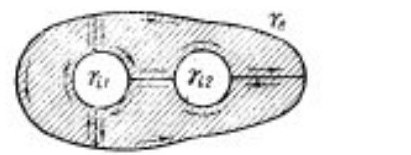
\includegraphics[width=130pt,keepaspectratio]{picc2}
        \vspace{19pt}
        \textit{\caption{}}
        \end{minipage}
        \end{figure}

    Функции $P$ и $Q$, как и выше, предполагаются непрерывными \linebreak вместе со своими производными $\dfrac{\partial P}{\partial y}$ и $\dfrac{\partial Q}{\partial x}$ в замкнутой области $\overline{G}$. \par

    Доказывается эта формула так же, как и формула (47.12), если \linebreak только заметить, что в сумме, стоящей в правой части равенства \linebreak (47.17), остаются криволинейные интегралы по положительно \linebreak ориентированным частям внешнего контура и по отрицательно ори- \linebreak ентированным частям внутренних контуров (рис. 151). \par
    Отметим еще, что в формуле (47.19) все контуры (как внешние, так \linebreak и внутренние) ориентированы таким образом, что при их обходе \linebreak область интегрирования остается слева. \par

    \textit{\textbf{Определение 7.} Пусть граница $\partial G$ ограниченной плоской \linebreak области $G$ состоит из конечного числа простых кусочно-гладких \linebreak контуров. Совокупность этих контуров, оринтированных так, что \linebreak при обходе по каждому из них область $G$ остается слева (справа), \linebreak называется положительной (отрицательной) ориентацией границы $G$ \linebreak и обозначается также $\partial G$ (соответственно --- $\partial G$).} \par

    Формулу Грина можно распространить и на еще более широкий \linebreak класс областей. Для этого заметим, что в силу доказанного формула \linebreak Грина справедлива для треугольника, а значит, и для любого много- \linebreak угольника. Поэтому предельным переходом, аппроксимируя границу \linebreak конечнозвенными ломаными, можно получить формулу Грина для \linebreak любой области (и даже просто открытого множества), граница ко- \linebreak}


\end{document}
